\documentclass{article}
% if you need to pass options to natbib, use, e.g.:
%     \PassOptionsToPackage{numbers, compress}{natbib}
% before loading neurips_2020

% ready for submission
\usepackage{neurips_2020}

% to compile a preprint version, e.g., for submission to arXiv, add add the
% [preprint] option:
% \usepackage[preprint]{neurips_2020}

% to compile a camera-ready version, add the [final] option, e.g.:
% \usepackage[final]{neurips_2020}

% to avoid loading the natbib package, add option nonatbib:
% \usepackage[nonatbib]{neurips_2020}

\usepackage[utf8]{inputenc} % allow utf-8 input
\usepackage[T1]{fontenc}    % use 8-bit T1 fonts
\usepackage{hyperref}       % hyperlinks
\usepackage{url}            % simple URL typesetting
\usepackage{booktabs}       % professional-quality tables
\usepackage{amsfonts}       % blackboard math symbols
\usepackage{nicefrac}       % compact symbols for 1/2, etc.
\usepackage{microtype}      % microtypography

% I need some pictures
\usepackage{float}
\usepackage{graphicx}
\graphicspath{ {.} }

% We have some very large tables and need to make them a bit smaller
\usepackage{tabularx}
\usepackage[table]{xcolor}

% Resnet
\usepackage{wrapfig}

\title{Model Stitching: Looking For Functional Similarity Between Representations}

% The \author macro works with any number of authors. There are two commands
% used to separate the names and addresses of multiple authors: \And and \AND.
%
% Using \And between authors leaves it to LaTeX to determine where to break the
% lines. Using \AND forces a line break at that point. So, if LaTeX puts 3 of 4
% authors names on the first line, and the last on the second line, try using
% \AND instead of \And before the third author name.

\author{Adriano Hernandez, Rumen Dangovski \& Peter Y. Lu\\
MIT EECS\\
Cambridge, MA 02139, USA \\
\texttt{\{adrianoh,rumenrd,lup\}@mit.edu}
}
\begin{document}

\maketitle

\begin{abstract}
  \textit{Model stitching} (Lenc \& Vedaldi 2015) is a compelling methodology to compare
  different neural network representations, because it allows us to measure to
  what degree they may be interchanged.
  We expand on a previous work from Bansal, Nakkiran \& Barak which used model stitching to
  compare representations of the same shapes learned by differently seeded
  and/or trained neural networks of the same architecture.
  Our contribution enables us to compare the representations learned by layers with
  different shapes from neural networks with different architectures.
  We subsequently reveal unexpected behavior of model stitching. Namely, we find that stitching, 
  based on convolutions, for small ResNets, can reach
  high accuracy if those layers come later in the first (sender) network than in
  the second (receiver), \textit{even if those layers are far apart}. 

  This leads us to hypothesize that stitches are not in fact learning to match the
  representations expected by receiver layers, but instead finding different representations which nonetheless
  yield similar results. Thus, we believe that model stitching may not necessarily always be an
  accurate measure of similarity.
\end{abstract}

\section{Introduction}
% NNs learn good reps
% We do not understand them
% We do not understand how to compare them
The success of deep learning for visual recognition has been attributed to the ability of neural networks to learn
good representations of their training data \cite{Rumelhart1986LearningIR}. That is, intermediate outputs (which we refer
to as ``representations'') of good neural networks 
are believed to encode meaningful information about their inputs, which these neural networks use for classification and/or other
downstream machine learning tasks \cite{goodfellow2016deep}.
However, our understanding of these representations is somewhat limited. Though
deep learning interpretability research, particularly for computer vision, has helped us
to intuitively grasp what deep neural 
networks are learning, we do not
know why good representations are learned, nor do we have a robust theory to characterize them. For example, we do not
know how to compare representations effectively.

% Our goal is to find functional similarity
% Define functional similarity
% Explain why functional similarity is good
% Papers do not find functional similarity
% We find functional similariy based on Bansal's work
%   - Bansal's work finds whether one thing can be translated into another
%   - If two things can easily be translated between we consider them to be functionality similar
%   - Thus they find functional similarity
%   - We expand their work for larger cases
Our goal is to improve the existing toolbox to find \textit{functional} similarity between representations.
% By functional similarity, we mean that two representations could be used in similar ways, which
% we believe is tightly coupled with them having similar information, even if that information is
% stored in vastly different ways. We believe this to be a salient measure of similarity, since
% it is practical and interpretable, using measures like task accuracy.
It is not obvious how to find functional similarity.
Many papers \cite{Kornblith2019SimilarityON} \cite{Morcos2018InsightsOR} \cite{Ding2021GroundingRS}
look for measures of statistical or geometric similarity because they can confirm known edge cases (i.e. when
representations are exactly the same).
However, these measures are not very informative in general, since neural networks'
representations can vary greatly in ways which are not yet well-understood,
simply due to random initialization of the weights. 

We believe that a previous work \cite{Bansal2021RevisitingMS} provides us with such a measure. It uses,
learned transformations to \textit{translate} representations from one layer into those for another
layer. Their technique measures functional similarity, because invariant to the type of transformations used,
it tests whether two representations can be interchanged, which is a strong indicator that the two representations
function similarly. However, their work can only
compare representations with the same shapes.
We expand it to include all representations taking the form of
ResNet tensors with widths and heights that are multiples of each other.

\section{Experimental Setup}
\label{ExperimentalSetup}
\subsection{Models and Dataset}
We compare all different
layers of all ResNets with a number of layers ranging from ten to eighteen.
These ResNets are trained on CIFAR-10 for comparable results
with Bansal et. al. These small ResNets we characterize with 4-tuples, where 
each element is either one or two, representing the number of residual blocks per stage\footnote{
   Residual blocks are partitioned into four stages of consecutive blocks, within which they have the same shape. At each stage, the
   width and height halve, while the width doubles \cite{He2016DeepRL}.
}. Since we use at most two blocks per stage, we can denote these 4-tuples unambiguously as
$R_{1111}$, $R_{1112}$, and so on. There are $2^4 = 16$ such ResNets. Note that $R_{2222}$ is equivalent
to the well-known Resnet18 architecture, while $R_{1111}$ is equivalent to Resnet10.

\subsection{Experiment}
We train each possible Small Resnet on CIFAR-10, yielding an accuracy above 90\%. We also
generate a randomly initialized, untrained network for each Small Resnet architecture and confirm
that these have an accuracy of around 10\%\footnote{There are ten classes in CIFAR-10.}. All these
networks are frozen and cannot learn during stitching.

We stitch every ordered pair of Small Resnets. There are $16 \cdot 16 = 256$ such pairs.
In every ordered pair of networks being stitched, the former is called the \textit{sender}, and the latter
is the \textit{receiver}. A stitch is used to transform the output of the sender at an intermediate layer
before inputing it into an intermediate layer in the reciever. For any network $A$ we can consider 
layer $i$ as $A_i$, the first $i$  layers (assuming we start at zero) as $A_{<i}$, and the layers 
after $i$ as $A_{i<}$. If we wish to include layer $i$ we can always call such (partial) networks
$A_{\leq i}$ or $A_{i\leq}$. For an input $x$, if we call the sender $A$, the reciever $B$,
and the stitch $S$, we call $C = B_{j<}(S(A_{\leq i}(x)))$ the \textit{stitched network}. Normally,
we train $S$ by doing backpropagation on the stitched network with both $A$ and $B$ frozen. The
resulting accuracy is used to find the similarity between $A_{\leq i}(x)$ and $B_{\leq j}(x)$, the
former of which is called the \textit{provided representation} and the latter of which is called
the \textit{expected representation}.

Unlike Bansal et al., which only compare corresponding blocks (i.e. $i = j$) of a sender and
reciever with the same architecture,
we we stitch from \textit{all} residual blocks of the sender into
\textit{all} residual blocks of the receiver even when they have different architectures, as long as
they are Small Resnets. Also unlike Bansal et al., we only vary
our neural networks by their initialization weights, but our setup is otherwise nearly identical. To
be able to stitch between all blocks, we use strided convolutions or upsampling when the dimensions
are not the same.
In our case the heights and widths vary by powers of two so we can simple use 2x2, 4x4,
or similarly-sized convolutions to downsample. For upsampling we use 2x, 4x, or similarly
sized 2D nearest-upsampling (meaning that an element is copied into a grid of equally-valued elements)
before applying a 1x1 convolution in the stitch.

We use the randomly-initialized ResNets as controls. Our controls enable us to make sure that
the stitches are appropriately powerful. By powerful we mean how complex the functions are that
stitches can represent. If a stitch is very powerful, then even with random networks it should be able to
yield high downstream accuracy because it can learn any transformation. In this case our 
stitches would always yield high ``similarity'' (downstream accuracy) and therefore be uninformative.
We can be sure this is not the case by ensuring that
the stitches never yield high similarity for random networks (where only overly powerful stitches
would).

\begin{center}
  \begin{figure}[H]
     \centering
     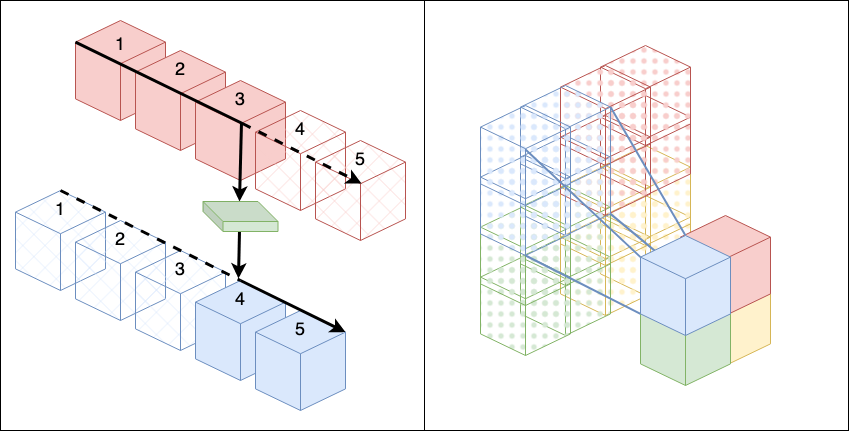
\includegraphics[width=12cm]{stitch2d2.drawio.png}
     \caption{\textbf{On the left}, a diagram exemplifying a stitch from the red (sender) network into the blue (reciever) 
     network comparing layer 3 from both. In this diagram, the blue layer 3 is the expected representation. Unused layers
     in the stitched network are displayed as partially translucent. The stitch
     is depicted in green. The arrows denote the flow of computation. The dashed arrows denote the flow of computation
     in regular operation, absent of stitching. \textbf{On the right}, a diagram exemplifying a 2x2 convolution (downsampling)
     from left (dotted) to right (solid). A 2x2 convolution such as this one could be used to stitch from a representation with 
     larger width and height to one of smaller dimensions. The colors are  chosen so as to elucidate which elements correspond.
     The blue lines further highlight the correspondence for the blue elements.
     In the case of upsampling, the image can be read from right (solid) to left (dotted), where the solid blue 
     element is copied four times to the
     dotted blue elements before it is used (later) for a 1x1 convolution.}
  \end{figure}
\end{center}

\section{Results}
\label{Results}
For every ordered pair of networks, we plot the accuracy of all the stitched networks on a grid,
based on the sender's layer and the receiver's layer. The layer is
denoted by an integer which counts how many residual blocks came before it\footnote{
   The initial convolution is ``0,'' the first block of the first stage is ``1,'' and so on.
}. The value in the grid element is the accuracy of the stitched network after traning. Thus, this
grid is a \textit{similarity matrix} where entry $i, j$ correspnds to the similarity of
$A_{\leq i}(x)$ and $B_{\leq j}$.

\subsection{Expectations}
We hypothesized that for similarity matrices between networks of the same architecture we would
see a high similarity diagonal. For networks of different architectures we hoped for a shorter diagonal
(since the matrix isn't square) or a diagonal with a different slope.

Generally, however, we assumed
that there would exist some non-negligible number $\epsilon$ such that if we mapped each
sender layer's representation to its most similar counterpart in the reciever,
and their similarity was $s$, the similarity between that layer's representation 
in the sender and every other layer's in the reciever would be
less than $s - \epsilon$. Moreover, we assumed that such a mapping would be injective. Intuitively,
we thought that there would be a one-to-one correspondence between most layers in the sender
to most layers in the reciever. We did not expect any layers' representation in the sender to have 
high similarity to \textit{multiple} layers' representations in the reciever.

These hypotheses make sense because Bansal et. al.'s findings suggest that each layer in the sender
should have at least one similar layer in the reciever---at least in the cast of identical architectures,
where those two layers are the corresponding ones; and it is usually assumed that distant layers
have different information, and so they should not be similar. However, \textbf{we found that every
layer in the sender was extremely similar to all layers before it in the reciever}. That is to say,
regardless of the architecture, if $j \leq i$ then the similarity was high. Visually, this looks
like a triangle in the lower left-hand corner of the similarity matrix. This is visible in the figure
below and quite perplexing.

For our controls we expected to see low stitching accuracy throughout the board since the networks are random,
and we did. With that said, some of the top left or bottom right elements have high similarity depending on
whether the sender or reciever was random. In the case of a random sender and trained reciever, if $i$ and $j$
are small, it is easy for $S$ to undo $A_{\leq i}$, and give $B_{j<}$ something usable. The opposite
case is analogous.

\begin{center}
   \begin{figure}[H]
      \centering
      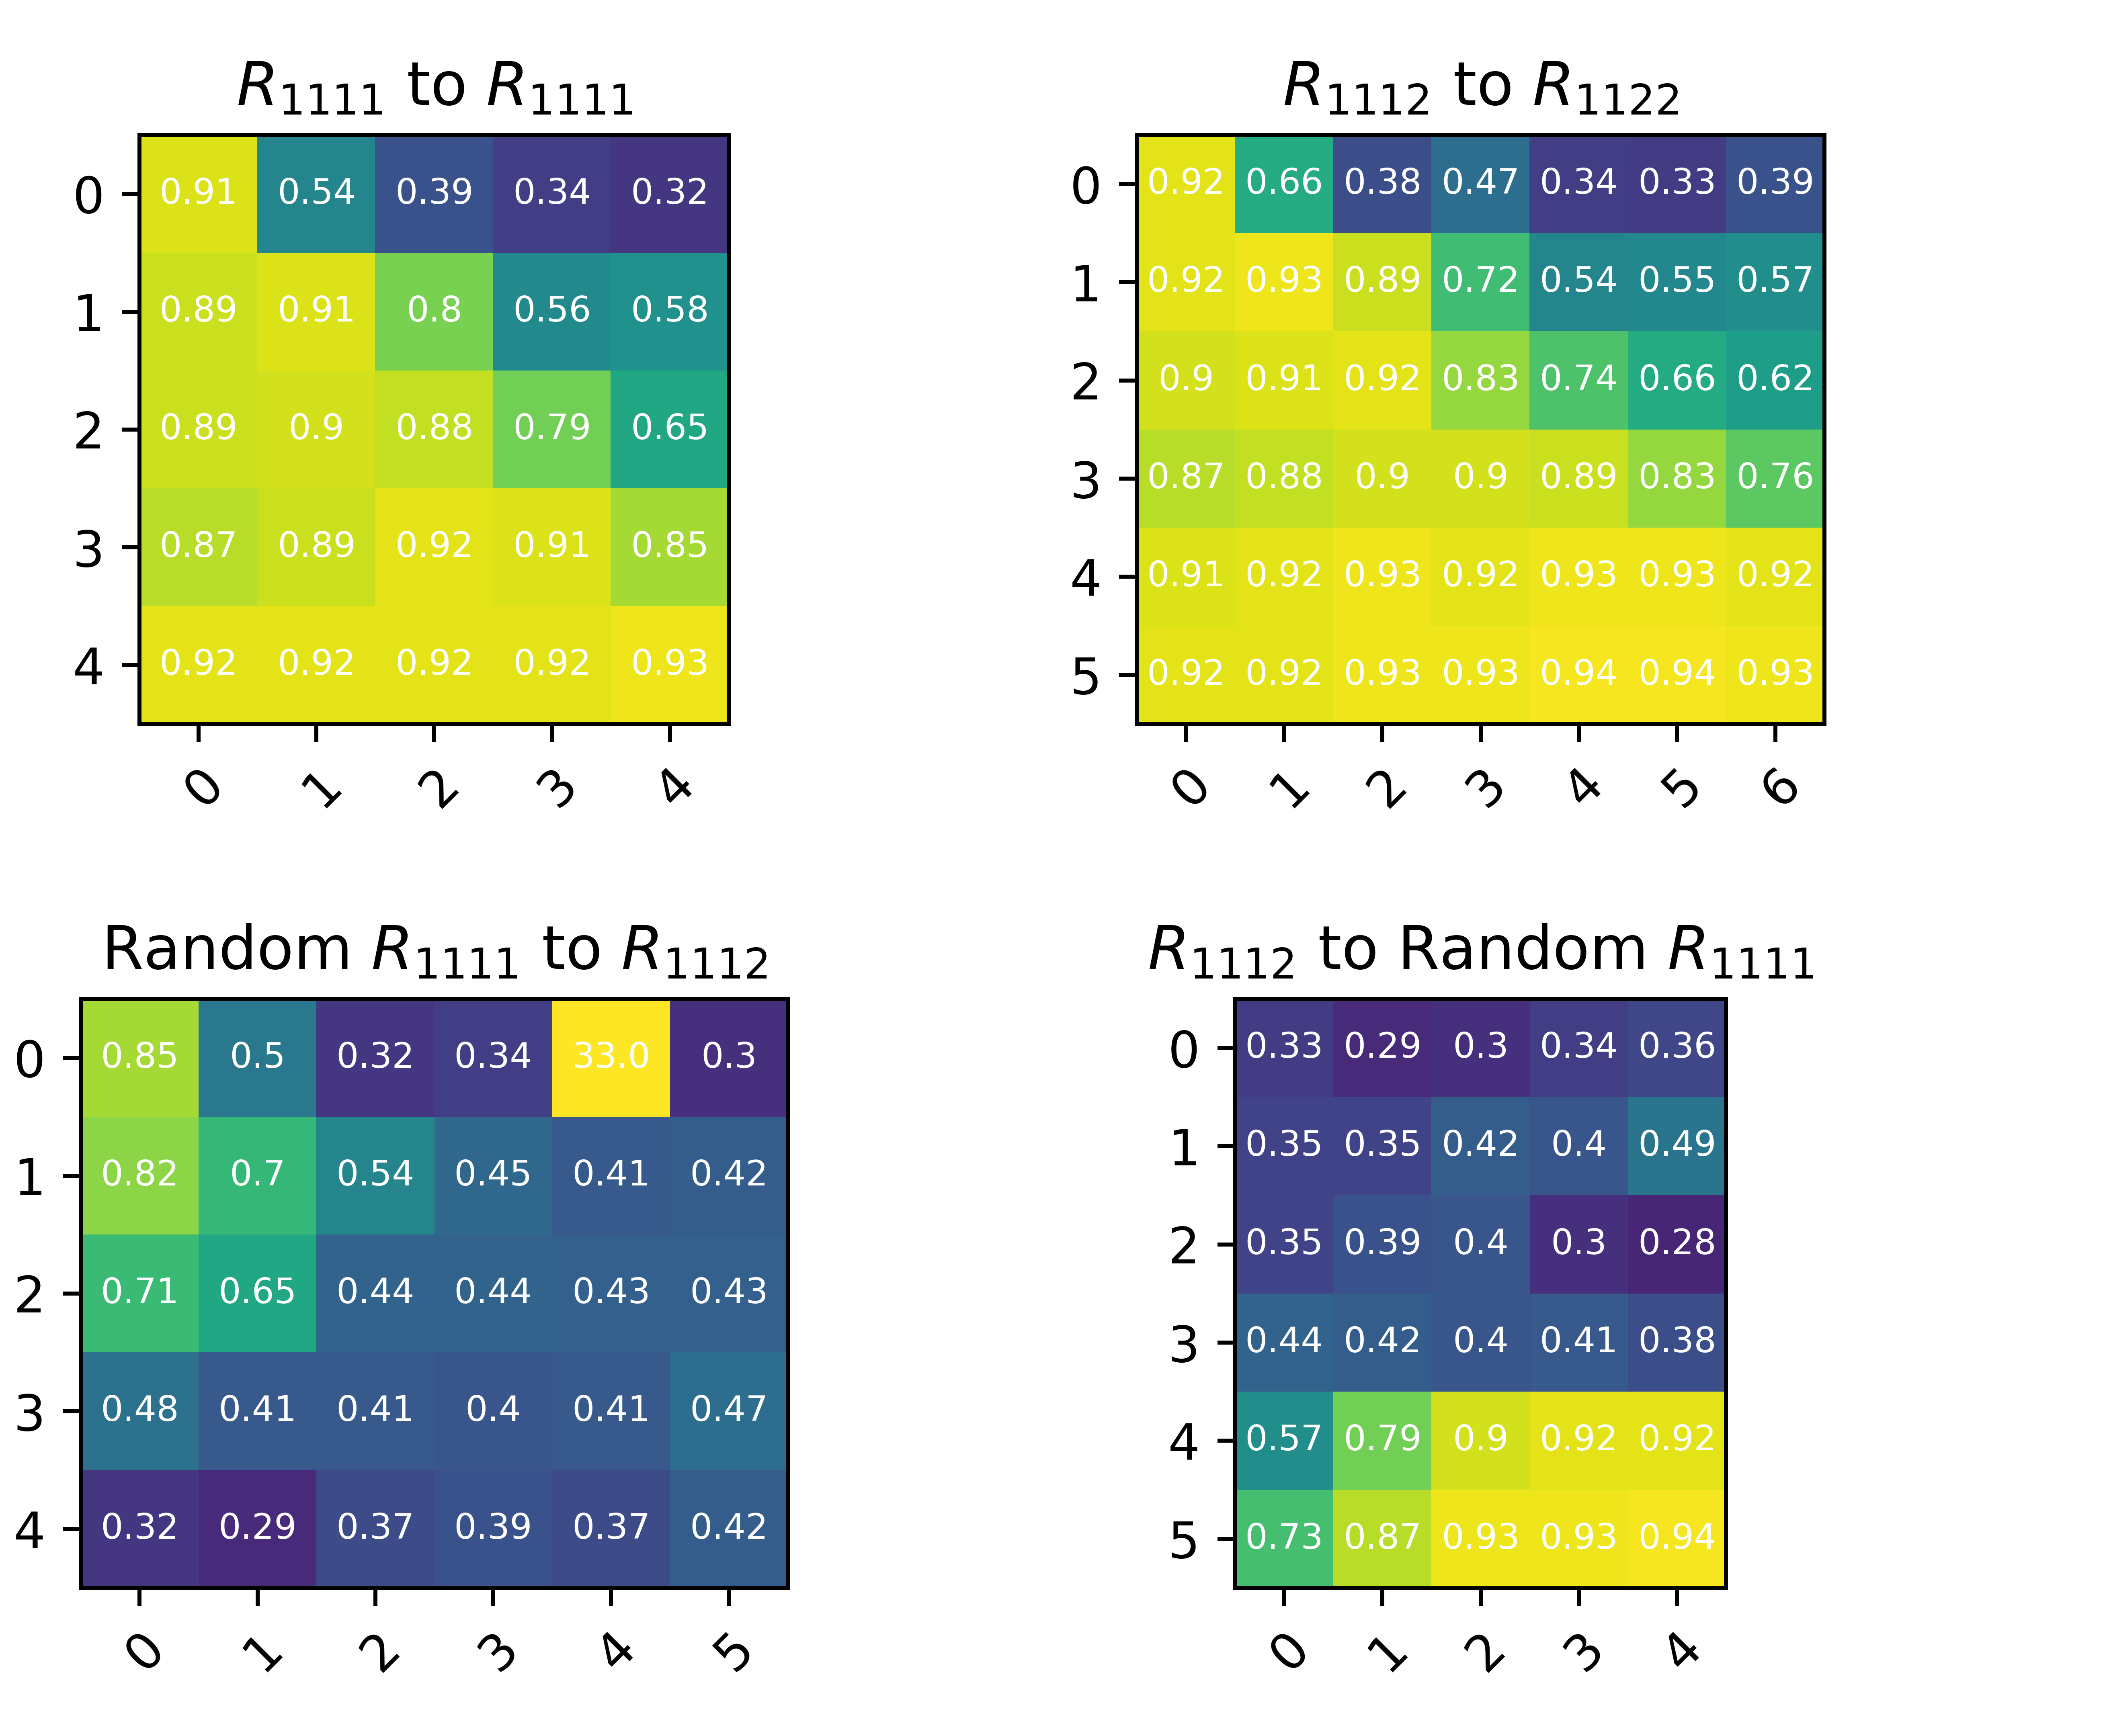
\includegraphics{tables.png}
      \caption{Triangle similarity pattern between trained Small Resnets and (expected) low similarity pattern for
      random ones. The plot is to be interpreted as a similarity matrix from sender to reciever.}
   \end{figure}
\end{center}

\subsection{Conclusion}
The most interesting aspect of our results is the high accuracy of the stitching network
for layers in the lower left hand triangle. Given that we interpret the stitching network accuracy
as a similarity, our results suggest that each sender representation is similar with \textit{all}
the receiver representations from a layer before it. We expected to see that each layer would be
similar to a couple (nearby) layers at most because the standard narrative has been that 
every layer loses some amount of granular information, and so that information should not be reconstructable
in an \textit{interchangeability} test like stitching.

We see two main explanations for the results. The first is that the common narrative could be wrong and some neural
networks may in fact be able to maintain most if not all of the granular information of the image throughout their
processing of it. The second is that the stitch may be able to give the reciever a representation which, despite being
different from that which is expected, nonetheless yields high accuracy.

We believe that the latter option is the most likely. Intuitively, the stitch may be able to figure out how to
generate some generic, albeit unrealistic, set of the most salient features for the recieving layer to classify
in a given way. Perhaps it is generating the ``average'' human, for example. However, a deeper analysis is required
to ascertain whether that is the case. In the Appendix, we further discuss sanity tests we explored and dub this
hypothesis \textit{hacking}.

Despite our difficulty generalizing model stitching, we still see it as an important
step forward in our ability to compare representations, since its focus on
\textit{functional} similarity makes its results more salient than those from
geometric closeness or statistical measures. Unlike existing measures of similarity which
tend to look for literal distance between representations, stitching follows a process whereby
we define what behaviors should be exhibited by similar representations (i.e. they should
be interchangeable up to a degree of flexibility determined by the function class of the stitch)
and then devise tasks/experiments that test these behaviors on the representations under question.
This approach is far better, because the research community understands tasks much better than
the numerical, geometric, or statistical properties of representations. Moreover, it is
easier to interpret the resulting similarity measurements in terms of accuracy or other such
\textit{functional} quantities, making techniques like stitching more useful, even in practice.
We hope to see more
representational comparison techniques following the high-level process outlined above in the future.

\begin{ack}
Thank you to MIT EECS for funding this project and MIT SuperUROP and the Soljacic Lab for supporting it.
\end{ack}

% Ripped this shit from the .bbl in the iclr template ugh
\small
\begin{thebibliography}{6}
  \providecommand{\natexlab}[1]{#1}
  \providecommand{\url}[1]{\texttt{#1}}
  \expandafter\ifx\csname urlstyle\endcsname\relax
    \providecommand{\doi}[1]{doi: #1}\else
    \providecommand{\doi}{doi: \begingroup \urlstyle{rm}\Url}\fi
  
  \bibitem[Bansal et~al.(2021)Bansal, Nakkiran, and
    Barak]{Bansal2021RevisitingMS}
  Yamini Bansal, Preetum Nakkiran, and Boaz Barak.
  \newblock Revisiting model stitching to compare neural representations.
  \newblock In \emph{NeurIPS}, 2021.
  
  \bibitem[Ding et~al.(2021)Ding, Denain, and Steinhardt]{Ding2021GroundingRS}
  Frances Ding, Jean-Stanislas Denain, and Jacob Steinhardt.
  \newblock Grounding representation similarity with statistical testing.
  \newblock \emph{ArXiv}, abs/2108.01661, 2021.
  
  \bibitem[Goodfellow et~al.(2016)Goodfellow, Bengio, Courville, and
    Bengio]{goodfellow2016deep}
  Ian Goodfellow, Yoshua Bengio, Aaron Courville, and Yoshua Bengio.
  \newblock \emph{Deep learning}, volume~1.
  \newblock MIT Press, 2016.
  
  \bibitem[Kornblith et~al.(2019)Kornblith, Norouzi, Lee, and
    Hinton]{Kornblith2019SimilarityON}
  Simon Kornblith, Mohammad Norouzi, Honglak Lee, and Geoffrey~E. Hinton.
  \newblock Similarity of neural network representations revisited.
  \newblock \emph{ArXiv}, abs/1905.00414, 2019.
  
  \bibitem[Morcos et~al.(2018)Morcos, Raghu, and Bengio]{Morcos2018InsightsOR}
  Ari~S. Morcos, Maithra Raghu, and Samy Bengio.
  \newblock Insights on representational similarity in neural networks with
    canonical correlation.
  \newblock In \emph{NeurIPS}, 2018.
  
  \bibitem[Rumelhart et~al.(1986)Rumelhart, Hinton, and
    Williams]{Rumelhart1986LearningIR}
  David~E. Rumelhart, Geoffrey~E. Hinton, and Ronald~J. Williams.
  \newblock Learning internal representations by error propagation.
  \newblock 1986.

  \bibitem[Frankle \& Carbin(2018)Frankle and
    Carbin]{LotteryTicket}
  Jonathan Frankle and Michael Carbin.
  \newblock The lottery ticket hypothesis: Finding sparse, trainable neural
    networks.
  \newblock 2018.
  \newblock \doi{10.48550/ARXIV.1803.03635}.
  \newblock URL \url{https://arxiv.org/abs/1803.03635}.

  \bibitem[He et~al.(2016)He, Zhang, Ren, and Sun]{He2016DeepRL}
  Kaiming He, X.~Zhang, Shaoqing Ren, and Jian Sun.
  \newblock Deep residual learning for image recognition.
  \newblock \emph{2016 IEEE Conference on Computer Vision and Pattern Recognition
    (CVPR)}, pp.\  770--778, 2016.

  \end{thebibliography}
\newpage
\appendix
\section{Appendix}
Here we provide additional information that may be helpful to readers, but which was
beyond the scope of the main paper. There are three subsections: further details on our
testing procedures; results from larger Resnets to support the idea that our surprising findings
could generalize; and numerical sanity testing to try and confirm or disprove the \textit{hacking}
hypothesis.
%; and images, generated using stitches (into the first layer), also to try and
% confirm or disprove the \textit{hacking} hypothesis. Unfortunately, neither of these latter
% two experimental results can definitively tell us what is going on.
\subsection*{Experimental Details}
% Wrapping is unfortuantely retarded and unusable.... we need a better way to do this
% \begin{wrapfigure}[35]{l}{3cm}
%   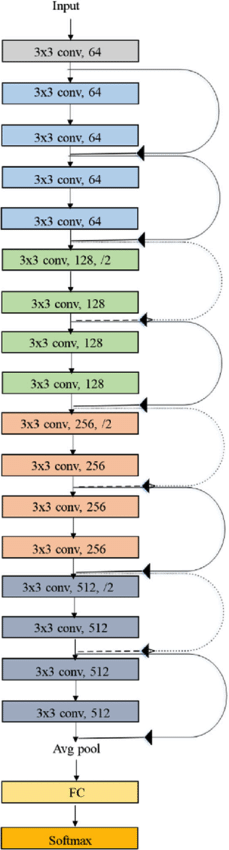
\includegraphics[width=3cm]{resnet18-arch.png} 
%   \caption{Resnet18 \cite{He2016DeepRL}}
% \end{wrapfigure}
We train our stitches for four epochs with momentum 0.9,
batch size 256, weight decay 0.01, learning rate 0.01, and 
a post-warmup cosine learning rate scheduler. We chose our
hyperparameters because they were effective for training the
Small Resnets between which we stitched. Below is an example of
a Small Resnet for clarity on our architecture.
\begin{center}
  \begin{figure}[H]
     \centering
     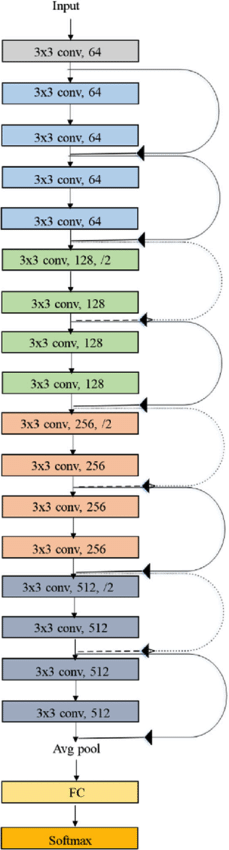
\includegraphics[width=3cm]{resnet18-arch.png}
     \caption{Resnet18 \cite{He2016DeepRL}, equivalent to $R_{2222}$
     using our nomenclature.}
  \end{figure}
\end{center}
\subsection*{Extrapolation to Larger Resnets}
\begin{center}
  \begin{figure}[H]
     \centering
     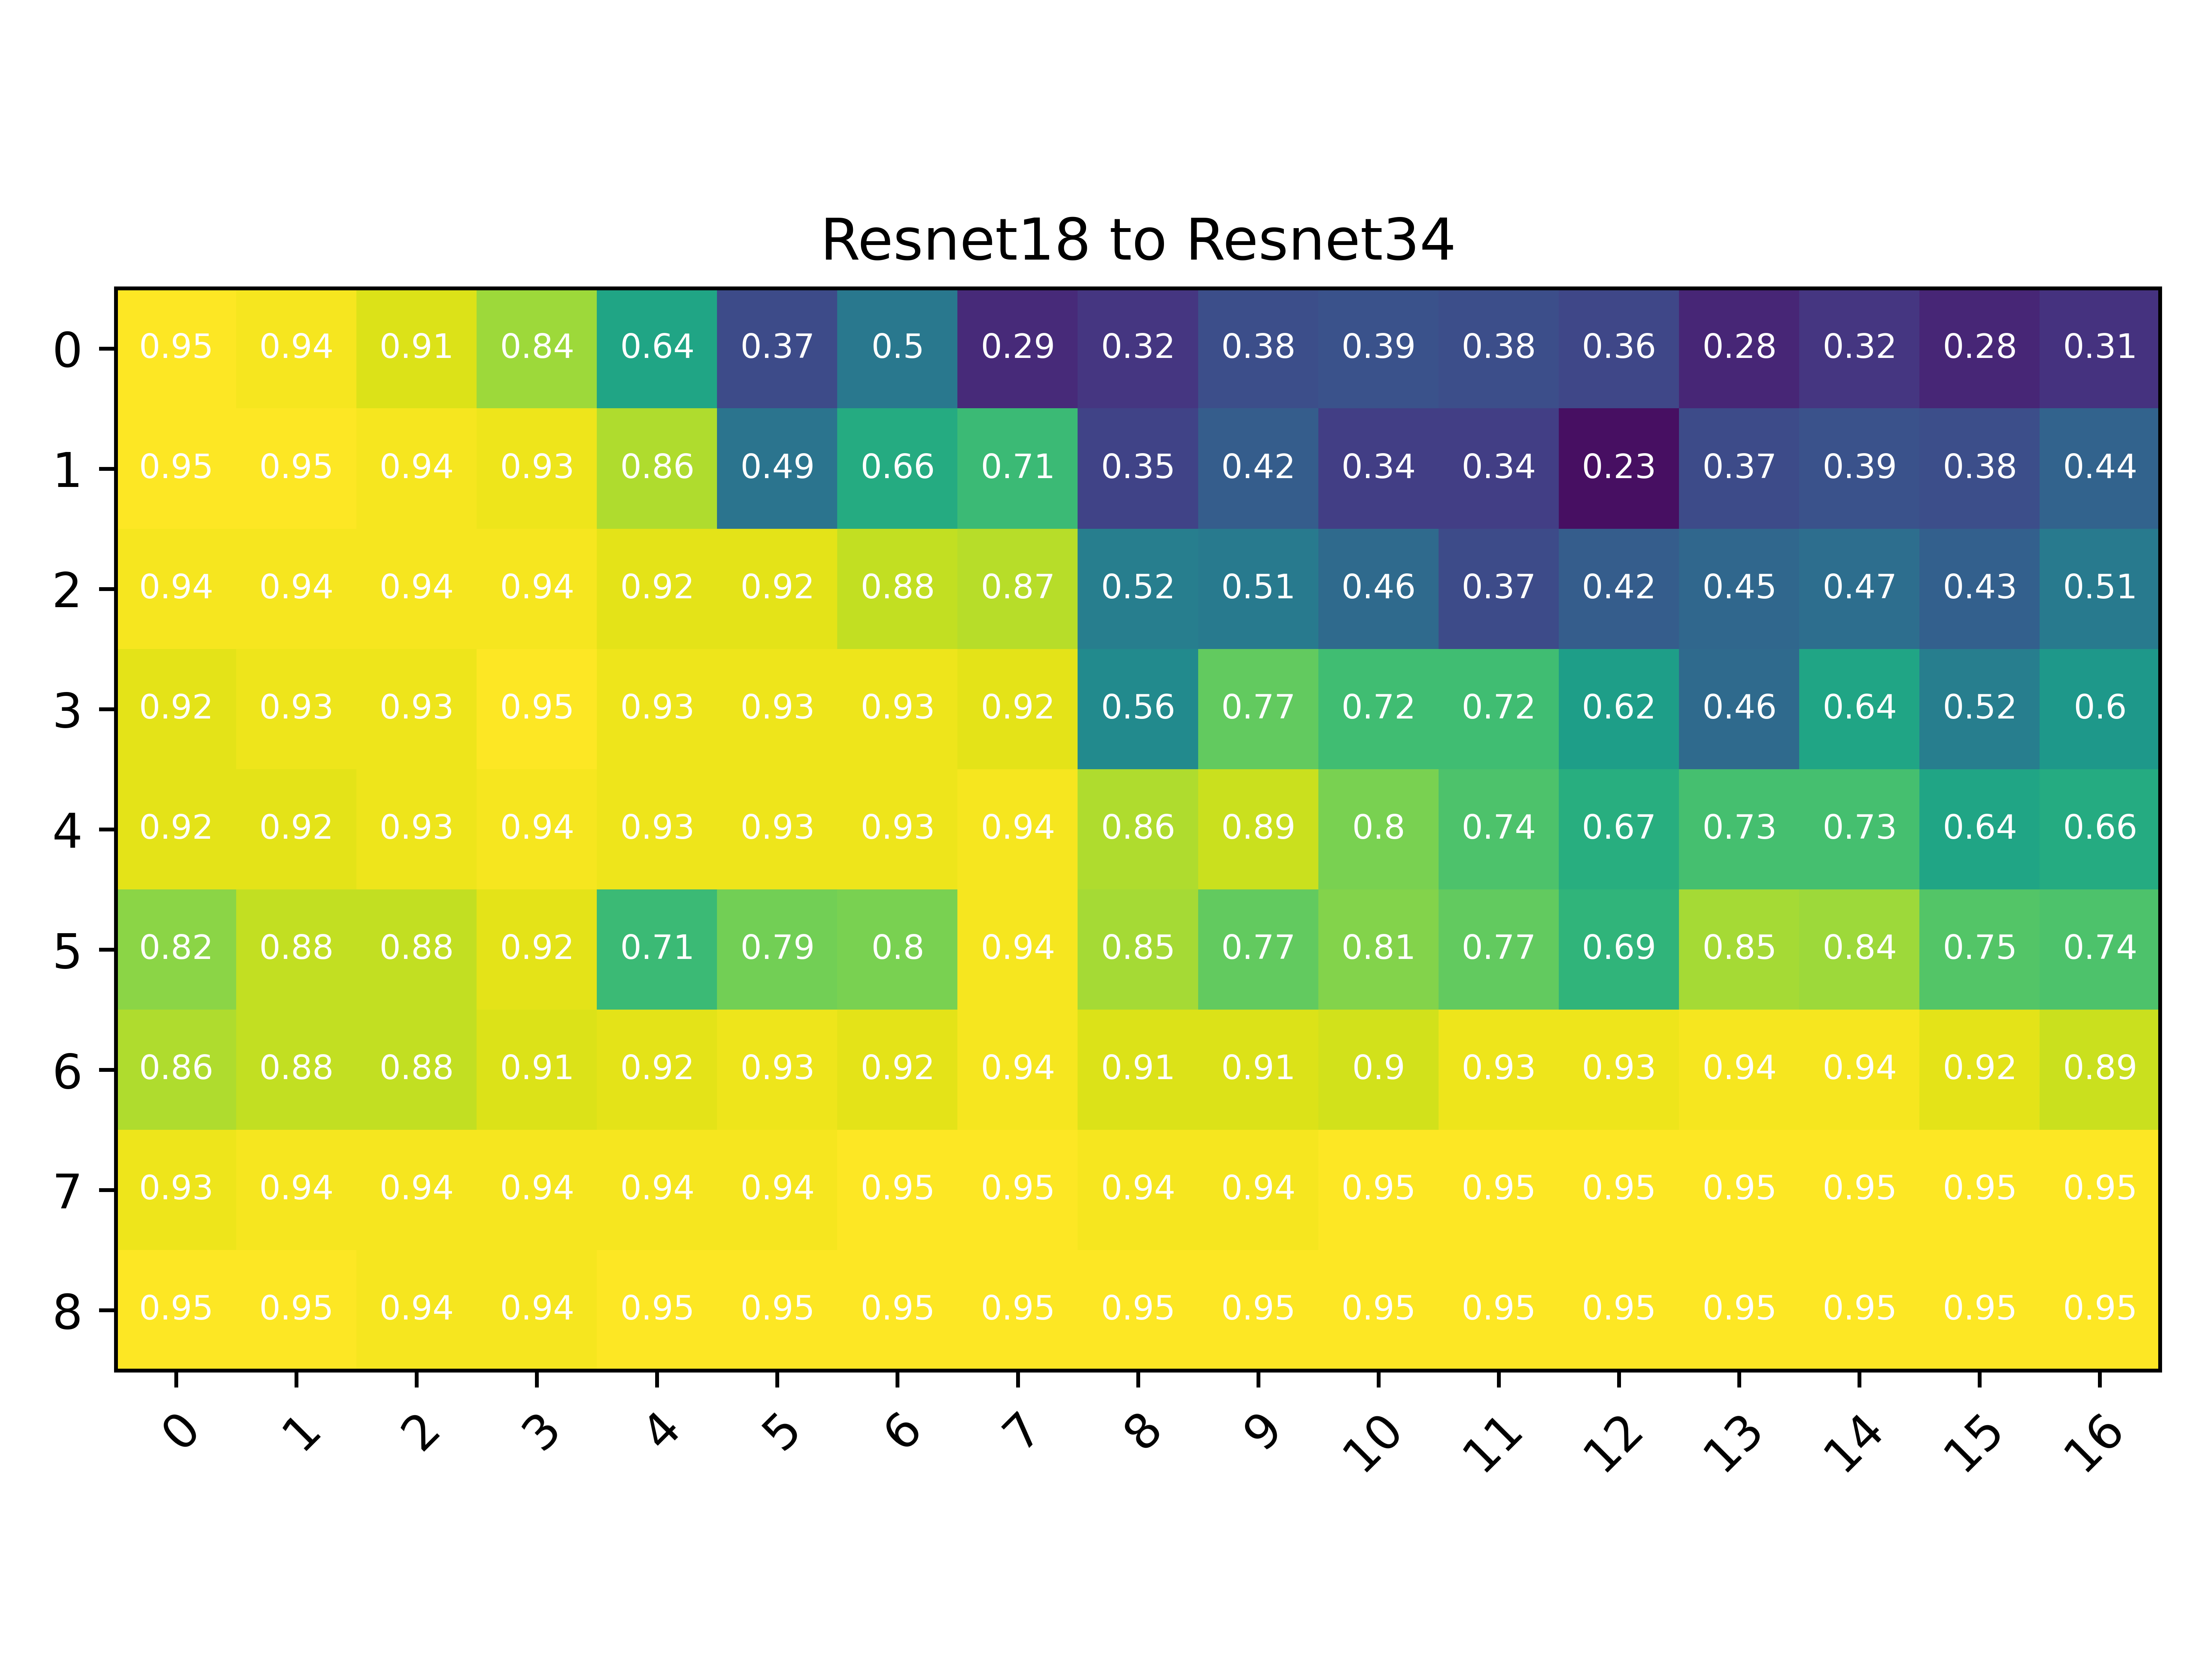
\includegraphics[width=14cm]{bigboi.png}
     \caption{Our results generalize to larger Resnets of a similar type (also on CIFAR-10).
     We were able to yield the same triangular pattern between Resnet18 and Resnet34 in both
     directions, suggesting that our results are the function of some general property of the
     Resnet architecture or of CIFAR-10.}
  \end{figure}
\end{center}
\subsection*{Numerical Sanity Testing}
When we found that our metric was finding high similarity between distant layers, we decided to sanity test
this result using numerical testing. We averaged the mean squared error between three pairs of values:
the expected representation with that generated by a vanilla stitch (trained with backpropagation on the CIFAR-10
classification task, as discussed in the body of this paper); the expected representation with that generated 
by a similarity-trained stitch; and the representation generated by similarity-trained stitch with that generated 
by a vanilla stitch. Respectively, we refer to these three pairs as \textbf{EV}, \textbf{ES}, and \textbf{SV}.
The mean squared error is over the elements in the representations' tensors. For those mean squared errors, we
found the minimum, mean, maximum, and standard deviation over the (cartesian product of the) entire dataset of
CIFAR-10 and all the pairs of layers across \textit{all} Small Resnets. We also measured the same statistics
for only corresponding layers (i.e. layer one with layer one) to get a baseline similar to what Bansal
et. al.'s work may have yielded.

Unlike the vanilla stitch, the similarity-trained stitch was trained to minimize the mean squared error between
the expected representation of the reciever (at a layer) and the output of the corresponding stitch. For example,
consider the input $x$, sender $A$, reciever $B$, and stitch $S$. Consider the stitched
network $C = B_{j<}(S(A_{\leq i}))$, and recall that the expected representation is $B_{\leq j}$ (that is, the computation
up to, including, layer $j$ of the reciever). The vanilla stitch would be trained using backpropagation on $C$ with
all the weights of $A$ and $B$ frozen (only the weights in $S$ can change). However, the similarity-trained stitch
would be trained on $(S(A_{<i}) - B_{\leq j})^2$. The purpose of the similarity-trained stitch is to get a baseline for
what a ``low'' mean squared error is. We include its task accuracy at the end of this section as a curiosity.

Below we plot our results in two tables. We denote the highest difference with red, that with the second highest 
difference with yellow, and that with the lowest difference with green. We expect, therefore, to see red in the
\textbf{EV} and \textbf{SV} columns and green in the \textbf{ES} column. That is because the similarity-trained
stitch should be closer to the expected representation (since the their difference is its loss function) than
the vanilla stitch is to either. If the vanilla stitch is learning to hack the reciever then we expect its
difference to be larger by many orders of magnitude than the similarity-trained stitch. While we do see that
our prediction is typically correct, the difference is not as large nor as decimatingly common as we had hoped,
and so we cannot conclude, from these results, that the stitch is likely hacking the reciever.
% (exp vs. vanilla), (exp. vs. sim), (sim vs. vanilla)
\begin{table}[ht!]
   \small
   \caption{Diagonals\strut}
   \scriptsize
   \begin{tabularx}\linewidth{||X|X|X||X|X|X||X|X|X||X|X|X|| }
      \hline
      \multicolumn{3}{||c||}{Minimum} & \multicolumn{3}{c||}{Mean} & \multicolumn{3}{c||}{Maximum} & \multicolumn{3}{c||}{Standard Deviation} \\
      \hline
      \textbf{EV}&\textbf{ES}&\textbf{SV}&\textbf{EV}&\textbf{ES}&\textbf{SV}&\textbf{EV}&\textbf{ES}&\textbf{SV}&\textbf{EV}&\textbf{ES}&\textbf{SV} \\
      \hline
      \cellcolor[HTML]{F8CECC}{\color[HTML]{000000}2.0e-3}&\cellcolor[HTML]{D5E8D4}{\color[HTML]{000000}2.2e-5}&\cellcolor[HTML]{FFF2CC}{\color[HTML]{000000}1.2e-3} & \cellcolor[HTML]{F8CECC}{\color[HTML]{000000}4.4e-2}&\cellcolor[HTML]{D5E8D4}{\color[HTML]{000000}1.5e-2}&\cellcolor[HTML]{FFF2CC}{\color[HTML]{000000}2.3e-2} & \cellcolor[HTML]{F8CECC}{\color[HTML]{000000}2.8e-1}&\cellcolor[HTML]{FFF2CC}{\color[HTML]{000000}1.9e-1}&\cellcolor[HTML]{D5E8D4}{\color[HTML]{000000}1.1e-1} & \cellcolor[HTML]{F8CECC}{\color[HTML]{000000}6.1e-2}&\cellcolor[HTML]{D5E8D4}{\color[HTML]{000000}3.7e-2}&\cellcolor[HTML]{FFF2CC}{\color[HTML]{000000}3.9e-2} \\
      \hline
      \cellcolor[HTML]{F8CECC}{\color[HTML]{000000}1.3e-1}&\cellcolor[HTML]{FFF2CC}{\color[HTML]{000000}5.5e-2}&\cellcolor[HTML]{D5E8D4}{\color[HTML]{000000}2.7e-3} & \cellcolor[HTML]{F8CECC}{\color[HTML]{000000}4.3e+5}&\cellcolor[HTML]{D5E8D4}{\color[HTML]{000000}7.6e+4}&\cellcolor[HTML]{FFF2CC}{\color[HTML]{000000}1.7e+5} & \cellcolor[HTML]{F8CECC}{\color[HTML]{000000}4.2e+6}&\cellcolor[HTML]{D5E8D4}{\color[HTML]{000000}3.6e+5}&\cellcolor[HTML]{FFF2CC}{\color[HTML]{000000}3.7e+6} & \cellcolor[HTML]{F8CECC}{\color[HTML]{000000}1.1e+6}&\cellcolor[HTML]{D5E8D4}{\color[HTML]{000000}1.3e+5}&\cellcolor[HTML]{FFF2CC}{\color[HTML]{000000}7.3e+5} \\
      \hline
      \cellcolor[HTML]{F8CECC}{\color[HTML]{000000}1.5e-2}&\cellcolor[HTML]{D5E8D4}{\color[HTML]{000000}3.5e-5}&\cellcolor[HTML]{FFF2CC}{\color[HTML]{000000}7.9e-3} & \cellcolor[HTML]{F8CECC}{\color[HTML]{000000}3.5e-1}&\cellcolor[HTML]{D5E8D4}{\color[HTML]{000000}1.1e-3}&\cellcolor[HTML]{FFF2CC}{\color[HTML]{000000}3.2e-1} & \cellcolor[HTML]{FFF2CC}{\color[HTML]{000000}5.3e-1}&\cellcolor[HTML]{D5E8D4}{\color[HTML]{000000}5.9e-3}&\cellcolor[HTML]{F8CECC}{\color[HTML]{000000}5.3e-1} & \cellcolor[HTML]{FFF2CC}{\color[HTML]{000000}1.6e-1}&\cellcolor[HTML]{D5E8D4}{\color[HTML]{000000}2.0e-3}&\cellcolor[HTML]{F8CECC}{\color[HTML]{000000}1.6e-1} \\
      \hline
      \cellcolor[HTML]{F8CECC}{\color[HTML]{000000}1.6e-1}&\cellcolor[HTML]{D5E8D4}{\color[HTML]{000000}1.7e-2}&\cellcolor[HTML]{FFF2CC}{\color[HTML]{000000}1.2e-1} & \cellcolor[HTML]{F8CECC}{\color[HTML]{000000}1.3e+2}&\cellcolor[HTML]{D5E8D4}{\color[HTML]{000000}4.9e+0}&\cellcolor[HTML]{FFF2CC}{\color[HTML]{000000}1.2e+2} & \cellcolor[HTML]{FFF2CC}{\color[HTML]{000000}1.4e3}&\cellcolor[HTML]{D5E8D4}{\color[HTML]{000000}6.0e+1}&\cellcolor[HTML]{F8CECC}{\color[HTML]{000000}1.4e+3} & \cellcolor[HTML]{FFF2CC}{\color[HTML]{000000}2.9e+2}&\cellcolor[HTML]{D5E8D4}{\color[HTML]{000000}1.3e+1}&\cellcolor[HTML]{F8CECC}{\color[HTML]{000000}2.9e+2}  \\
      \hline
   \end{tabularx}
   \medskip
   \small
   \caption{All Stitches\strut}
   \scriptsize
   % % (exp vs. vanilla), (exp. vs. sim), (sim vs. vanilla)
   \begin{tabularx}\linewidth{||X|X|X||X|X|X||X|X|X||X|X|X|| }
      \hline
      \multicolumn{3}{||c||}{Minimum} & \multicolumn{3}{c||}{Mean} & \multicolumn{3}{c||}{Maximum} & \multicolumn{3}{c||}{Standard Deviation} \\
      \hline
      \textbf{EV}&\textbf{ES}&\textbf{SV}&\textbf{EV}&\textbf{ES}&\textbf{SV}&\textbf{EV}&\textbf{ES}&\textbf{SV}&\textbf{EV}&\textbf{ES}&\textbf{SV} \\
      \hline
      % Template is \cellcolor[HTML]{#COLOR}{\color[HTML]{000000}#VALUE}
      % (Highest) Red: F8CECC
      % (Middle) Yellow: FFF2CC
      % (Lowest) Green: D5E8D4
      \cellcolor[HTML]{F8CECC}{\color[HTML]{000000}1.6e-3}&\cellcolor[HTML]{D5E8D4}{\color[HTML]{000000}5.4e-6}&\cellcolor[HTML]{FFF2CC}{\color[HTML]{000000}7.8e-4} & \cellcolor[HTML]{F8CECC}{\color[HTML]{000000}4.5e-2}&\cellcolor[HTML]{D5E8D4}{\color[HTML]{000000}1.6e-2}&\cellcolor[HTML]{FFF2CC}{\color[HTML]{000000}2.0e-2} & \cellcolor[HTML]{F8CECC}{\color[HTML]{000000}3.6e+0}&\cellcolor[HTML]{FFF2CC}{\color[HTML]{000000}1.3e+0}&\cellcolor[HTML]{D5E8D4}{\color[HTML]{000000}5.9e-1} & \cellcolor[HTML]{F8CECC}{\color[HTML]{000000}1.4e-1}&\cellcolor[HTML]{FFF2CC}{\color[HTML]{000000}5.9e-2}&\cellcolor[HTML]{D5E8D4}{\color[HTML]{000000}3.3e-2} \\
      \hline
      \cellcolor[HTML]{F8CECC}{\color[HTML]{000000}1.6e-4}&\cellcolor[HTML]{D5E8D4}{\color[HTML]{000000}1.7e-7}&\cellcolor[HTML]{FFF2CC}{\color[HTML]{000000}1.5e-4} & \cellcolor[HTML]{F8CECC}{\color[HTML]{000000}2.6e+5}&\cellcolor[HTML]{FFF2CC}{\color[HTML]{000000}1.1e+5}&\cellcolor[HTML]{D5E8D4}{\color[HTML]{000000}6.3e+4} & \cellcolor[HTML]{F8CECC}{\color[HTML]{000000}1.8e+7}&\cellcolor[HTML]{FFF2CC}{\color[HTML]{000000}9.2e+6}&\cellcolor[HTML]{D5E8D4}{\color[HTML]{000000}5.8e+6} & \cellcolor[HTML]{F8CECC}{\color[HTML]{000000}1.0e+6}&\cellcolor[HTML]{FFF2CC}{\color[HTML]{000000}4.3e+5}&\cellcolor[HTML]{D5E8D4}{\color[HTML]{000000}3.4e+5} \\
      \hline
      \cellcolor[HTML]{F8CECC}{\color[HTML]{000000}1.4e-2}&\cellcolor[HTML]{D5E8D4}{\color[HTML]{000000}6.3e-6}&\cellcolor[HTML]{FFF2CC}{\color[HTML]{000000}7.9e-3} & \cellcolor[HTML]{FFF2CC}{\color[HTML]{000000}2.2e+0}&\cellcolor[HTML]{D5E8D4}{\color[HTML]{000000}2.1e-3}&\cellcolor[HTML]{F8CECC}{\color[HTML]{000000}2.2e+0} & \cellcolor[HTML]{FFF2CC}{\color[HTML]{000000}2.3e+2}&\cellcolor[HTML]{D5E8D4}{\color[HTML]{000000}1.9e-2}&\cellcolor[HTML]{F8CECC}{\color[HTML]{000000}2.3e+2} & \cellcolor[HTML]{FFF2CC}{\color[HTML]{000000}1.2e+1}&\cellcolor[HTML]{D5E8D4}{\color[HTML]{000000}4.3e-3}&\cellcolor[HTML]{F8CECC}{\color[HTML]{000000}1.2e+1} \\
      \hline
      \cellcolor[HTML]{F8CECC}{\color[HTML]{000000}1.3e-1}&\cellcolor[HTML]{D5E8D4}{\color[HTML]{000000}1.6e-2}&\cellcolor[HTML]{FFF2CC}{\color[HTML]{000000}9.4e-2} & \cellcolor[HTML]{F8CECC}{\color[HTML]{000000}7.3e+4}&\cellcolor[HTML]{FFF2CC}{\color[HTML]{000000}4.2e+4}&\cellcolor[HTML]{D5E8D4}{\color[HTML]{000000}2.1e+4} & \cellcolor[HTML]{F8CECC}{\color[HTML]{000000}1.2e+7}&\cellcolor[HTML]{FFF2CC}{\color[HTML]{000000}6.9e+6}&\cellcolor[HTML]{D5E8D4}{\color[HTML]{000000}4.8e+6} & \cellcolor[HTML]{F8CECC}{\color[HTML]{000000}5.9e+5}&\cellcolor[HTML]{FFF2CC}{\color[HTML]{000000}3.4e+5}&\cellcolor[HTML]{D5E8D4}{\color[HTML]{000000}2.1e+5} \\
      \hline
   \end{tabularx}
\end{table}
\begin{center}
  \begin{figure}[H]
     \centering
     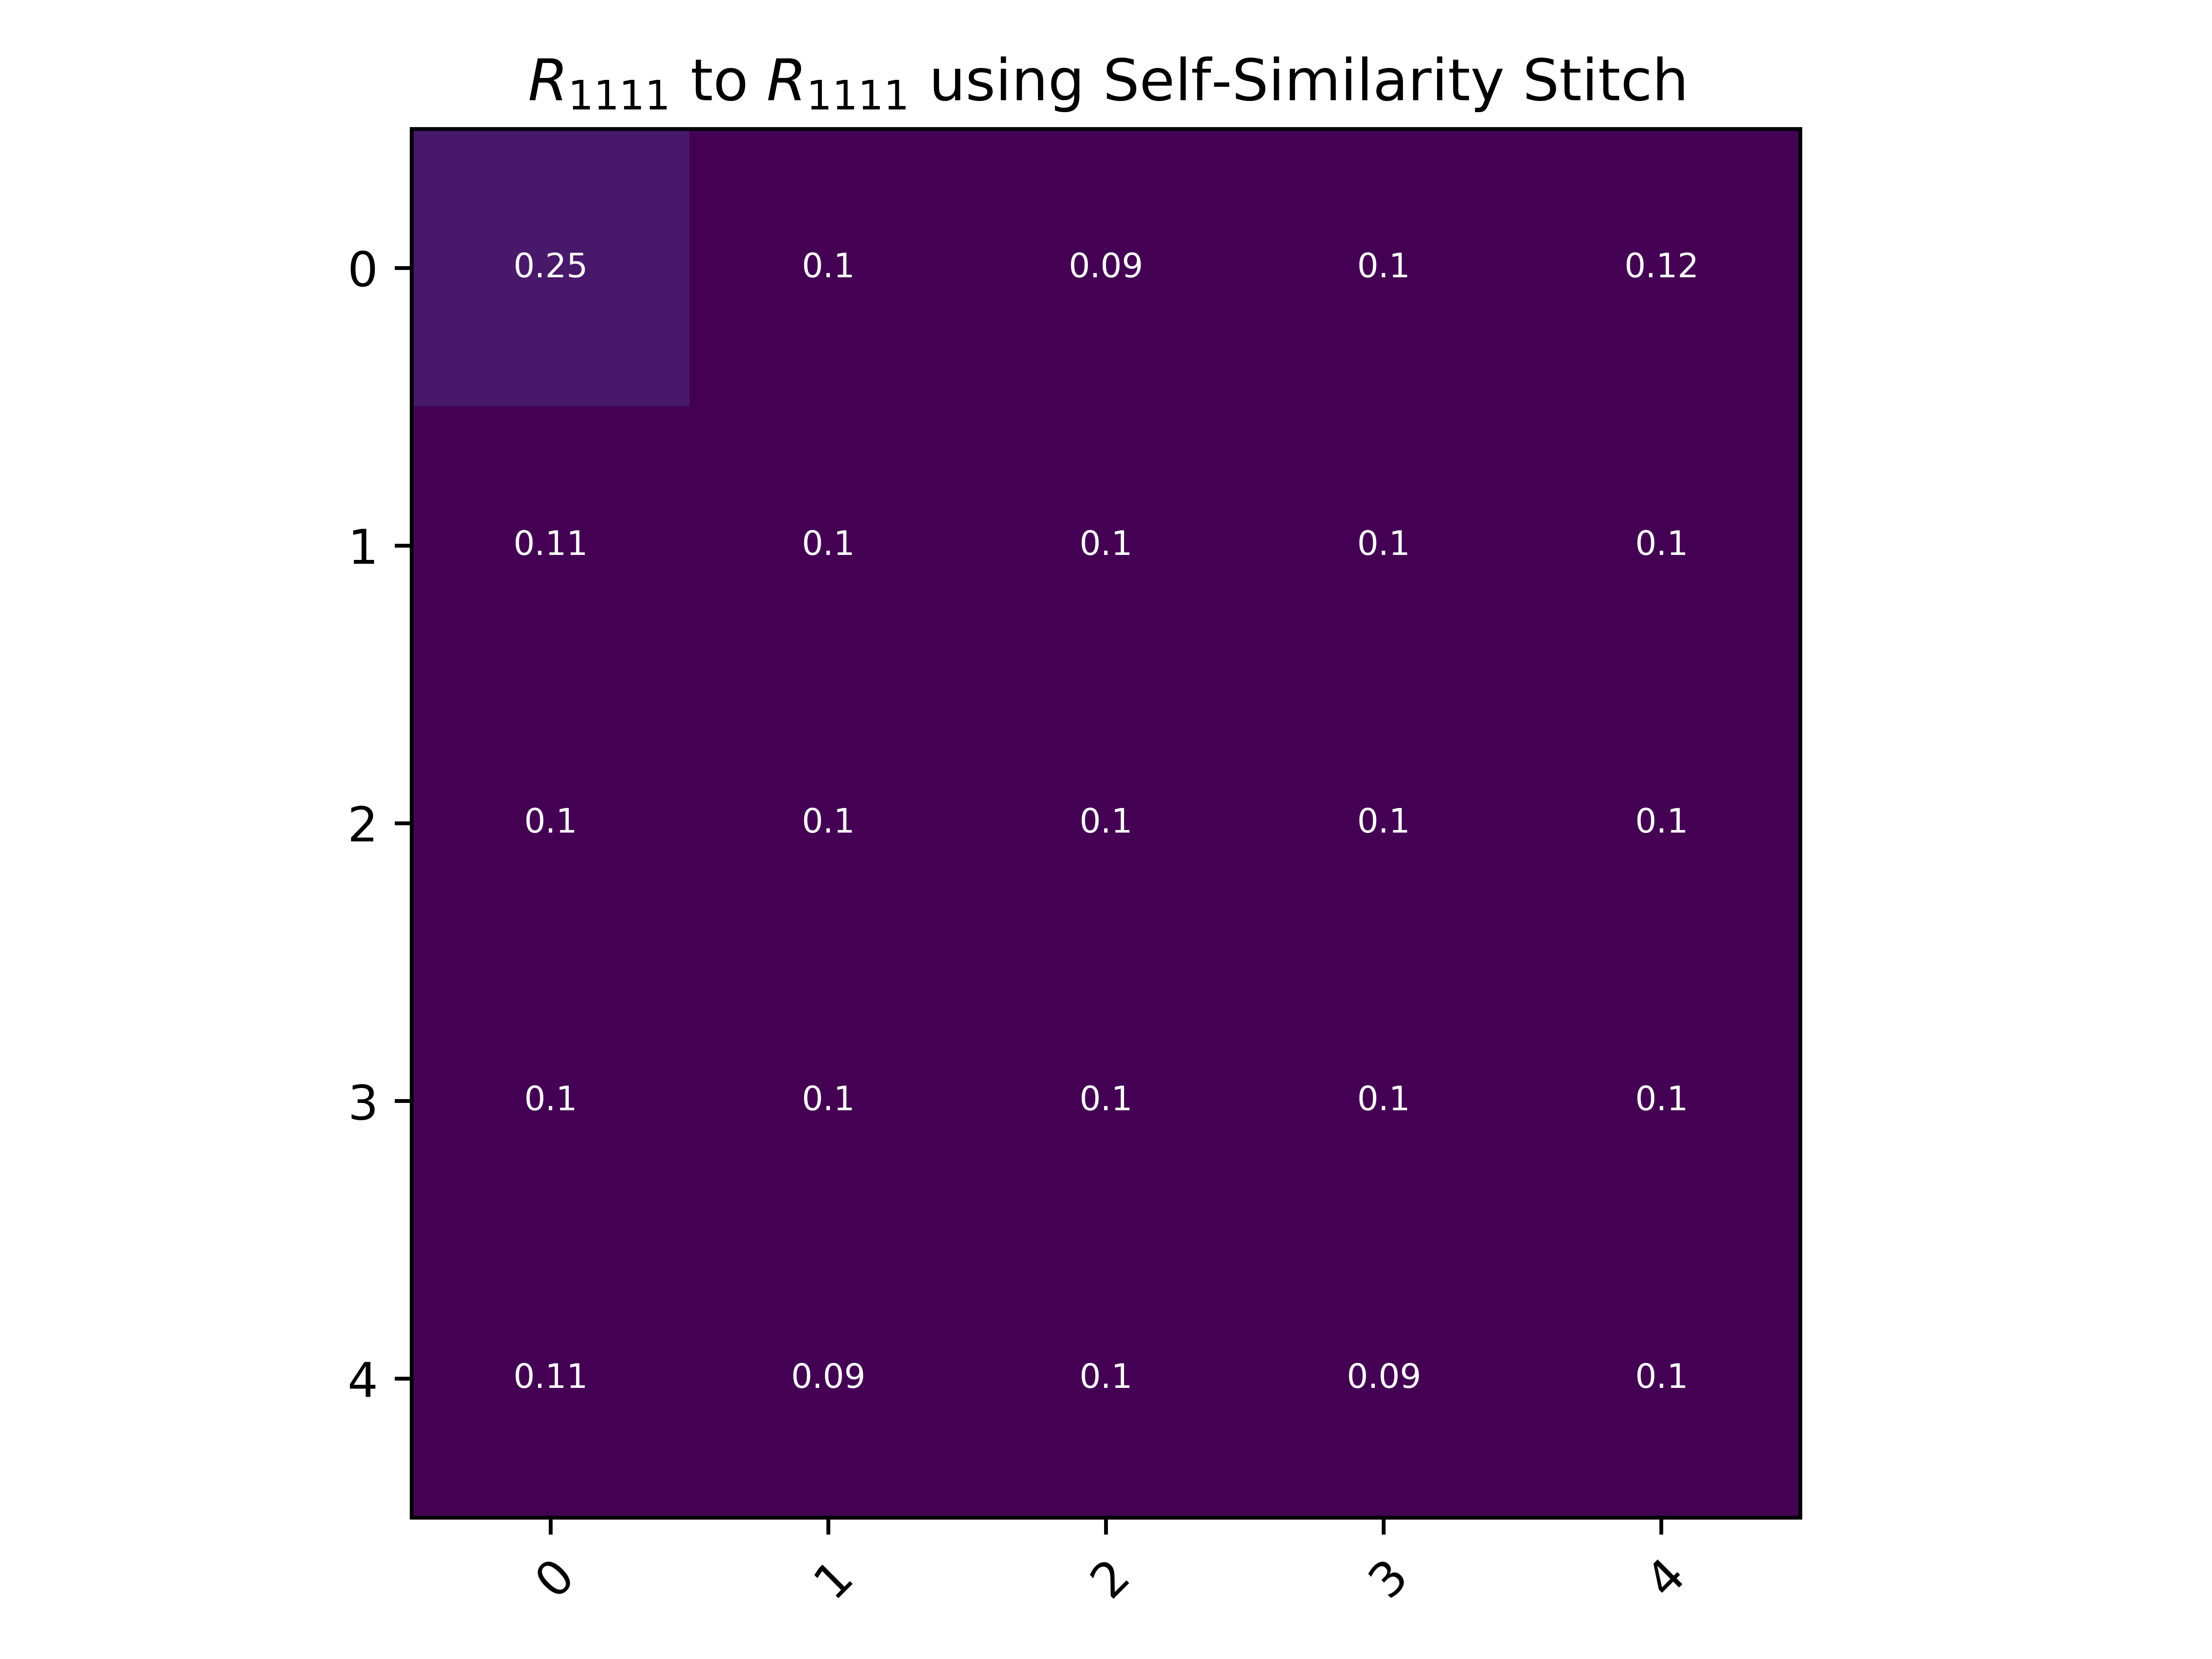
\includegraphics[width=14cm]{selfsim.png}
     \caption{We are unable to yield high task accuracy for stitched networks using
     similarity-trained stitches. This makes sense, since having no task information, it does
     not know what subspaces to prioritize. Most likely, only a few subspaces and/or weights
     truly matter for task accuracy, per the Lottery-Ticket hypothesis \cite{LotteryTicket}. Thus,
     not knowing which those are, the similarity-trained stitch cannot yield high task accuracy
     even when it is trained for thirty epochs to the vanilla stitch's four (the latter yielding
     a very high similarity near 90\% for the lower left-side triangle of the corresponding
     similarity matrix, per the previous figures in this paper).}
  \end{figure}
\end{center}
% This should be done.
% \subsection*{Image Generation}
% We tried generating images as a sanity test to see if we could shed some light on whether
% the Small Resnets' stitches were creating meaningful representations for their corresponding
% images. We stitched from all blocksets into the very first layer to do this. This approach
% makes sense for better understanding our results because images are human-interpretable, so
% we can get an intuitive sense of whether the stitch is creating meaningful outputs.
% However, unlike in other cases, the stitched network was only able to reach a maximum
% of around 30\%-40\% accuracy in this case. Perhaps the first layer of a Resnet is one of
% the most important ones. Regardless, the images were not very interpretable. Broad contours
% were maintained when stitching from earlier layers, but when stitching from later layers,
% it was difficult to find any pattern. Some sample images are below.
\end{document}
